\section{The Owl of Minerva}

\begin{quotex}
The owl of Minerva flies at dusk.

\end{quotex}
\paragraph{Seeing in the Dark}

\begin{wrapfigure}{tr}{.25\textwidth}
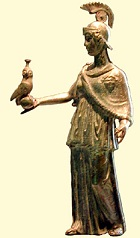
\includegraphics[scale=.9]{a20110630TheOwlofMinerva-img001.jpg} 
\end{wrapfigure}

This proverb from Hegel means that philosophy can only understand a cycle at its end. Hence, it is not helpful at its beginning, so anyone who is now engaged in the “battle of ideas” can hope for little more than a pyrrhic victory at best. Rather, it is a struggle of visions or world views. Pace Hegel, the Owl of Minerva is not a philosopher. The owl is wise not because he can think but rather because he can see in the darkness. While the world sleeps, the owl is vigilant at night. Thus, the men of Tradition must also be vigilant during the darkness.


At the beginning of a cycle, there is no need for philosophy. Man lives in immediacy following his Tradition faithfully and there is no need for questioning, and no need for wonder which is the motivation for philosophy. Unperturbed by the conflicts of competing thoughts, he lived with certainty. When an issue arose, he didn't think about it. Rather he followed the Tradition of his ancestors and his gods without question. His moral code was duty to the city, family, and gods. This code prescribed all his actions, which had to be executed precisely, and there was no room for subtleties. These rites maintained the souls of his ancestors and brought their blessings; he expected his sons to do the same for him after his death. These civilizations lived in relative internal harmony, sometimes for millennia.

Only with the decline of a cycle does thought arise. The corrosive effect of discursive thought calls everything into question. It no longer suffices to follow the ancestors and gods, one must also give a reason for doing so. Those skilled at logical and creative thinking become the philosophers. They offer their services to men in search of understanding. Others, such as the Sophists, notice that thought is an end in itself and can be used for persuasion apart from its actual truth value. The Sophists are the first propagandists and sell their services.

\paragraph{Three Civilizations}
\begin{quotex}
…bisogna tener ben fermo questo punto, indispensabile per una formulazione imperiale e romana dell'idea razzista e confermato da ciò che fu proprio alle grandi civiltà arie d'Oriente, all'antica Roma, al Medioevo romano-germanico.

\end{quotex}
We are focusing on the civilizations of the Borean race, as Fabre d'Olivet called it, who origins were in the mythical Hyperborea, whence it spread to India, Central Asia and Europe. There is not the time or energy to deal with the traditions of Asia, Africa, or the Amerindians. Furthermore, we have been focusing on just three Borean civilizations of a traditional nature, omitting the Nordic and Celtic traditions which are no less important. But since Julius Evola identified them as the three main civilizations of Indo-Eurpean origin, they serve as a good basis for discussion.

\begin{description}
\item[Hyperborea ]

We can get a glimpse into these people only through extrapolation. By the interpretation of myths we can try to reconstruct their society. For this, we are relying on \textbf{Bal Tilak}, \textbf{Fabre d'Olivet} and \textbf{Herman Wirth}. 

\item[Bharat Khant ]

Bharat Khant was the ancient name for the Vedic civilization of India. This is the oldest group that we have documentation for, which includes the Vedas and the Laws of Manu. It is most important for us today because of its rich metaphysical tradition which comprise the six orthodox schools, all deriving from the Vedas. This should not uncritically be confounded with the contemporary religion of Hinduism. Unlike Hinduism, the Vedic civilization included ancestor worship, animal sacrifice and rejection of reincarnation. 

\item[The Ancient City ]

By this, we mean the ancient city-states of Greece and Italy. Although their origins are obscure, their traditions and eventual decline are reasonably well documented. That makes their study invaluable to those of use seeking the light hidden by the darkness. 

\item[Christendom ]

Instead of circumlocutions such as “Medieval period” and the like, we will use this term to describe the civilization that arose in Europe following the fall of Rome, without intending by that term to impose a particular theological interpretation on it. To put a time frame on it, we mean the approximate thousand year reign from Constantine to the Reformation, which united spiritually much of Europe. We will see that it had its declines that mimicked the decline of the Ancient City, at least in principle if not in detail. But here we have the added advantage that its origins are also documented. Thus, we can see what it adapted from its predecessor and what it rejected. This will serve as a useful model for a new cycle. 

\end{description}
\paragraph{Three Types of Men}
Each period was marked by a special type of man who embodied its superior aspects. These were never theoretical men, or those with the “best idea”, but men of a higher knowledge, a direct knowing or gnosis that can never be fully encompassed in thought. The knowing took various forms.

\begin{description}
\item[The Seer ]

The type of the Vedic period was the \textbf{Rishi} and the \textbf{Yogi}. The Rishi, or seer, had clairvoyant vision to see into the nature or essence of things beyond the accidental, incidental, or the trivial. The Yogi was the man of power: for bhakti yoga, power over the emotions; for karma yoga, power over one's actions; for jnana yoga, power over one's mind. The jnani, or knower, was master of his mind. By transcending the stream of thoughts, which held no more significance to him than the movement of clouds across the sky, the jnani gained direct insight into the nature of things. 

\item[The Hero ]

The Hero of the Ancient City was the \textbf{Hero}, the patriarch of a family, the founder of the city. As priest, he was the link between the gods and men and had the power to invoke their blessings. As king, he had the power of command over men. He had the power to interpret the omens, because in order to predict the future, he had to create the future. 

\item[The Believer ]

Christendom began where the Ancient City left off, in particular, it separated the roles of priest and king, without, however, secularizing the latter as had been done in the successive revolutions of the previous era. This leads to two different figures, united in faith, although different in temperament. These are the Saint and the Knight. Rather than seeking godhood by means of the rituals and sacrifices of their sons as in the age of heroes, they relied on their respective devotions to the True God and the True Man. The \textbf{Saint} through his ascetical practices was drawn toward theosis (divinization). The \textbf{Knight} of heroic valor followed the path of the Fedeli d'Amore to lead to the alchemical marriage. 

\end{description}
\paragraph{The Way Forward}
\begin{quotex}
Io ho difeso e difendo idee … nella misura in cui riprendono una tradizione superiore e anteriore … in quanto appartengono al retaggio della carattere universale e mantenutasi in Europa fino all Rivoluzione francese. Nello stesso spirito … dei grandi filosofi cattolici del principio di autorità, de Maistre e Donoso Cortes … I miei principi sono solo quelli che prima della Rivoluzione francese ogni persona ben nata considerava sani e normali.

\end{quotex}
The way forward is indicated by Evola as quoted above: to defend the higher traditions of Europe that every well born person considered sane and normal. We need not look back to the distant past, just to Europe before 1789 since these principles have a universal character. To reject these principles, as those of the new right seem to do, is to squander our legacy and dishonor our ancestors. If anyone is unclear about those principles, please read Donoso Cortes’ essays\footnote{\url{https://www.gornahoor.net/library/CortesEssays.pdf}}, as Evola recommends.

The way forward is based on authority as illustrated by our examples. In future posts we will lay out some programs described by \textbf{Fabre d'Olivet} and \textbf{Saint-Yves d'Alveydre} based on theocracy, Synarchy and the spiritual unity of Europe. But ultimately, it will depend on men of vision, seers, heroes, and those of unshakable faith.

\flrightit{Posted on 2011-06-30 by Cologero}